% This work is licensed under the Creative Commons
% Attribution-NonCommercial-ShareAlike 4.0 International License. To view a copy
% of this license, visit http://creativecommons.org/licenses/by-nc-sa/4.0/ or
% send a letter to Creative Commons, PO Box 1866, Mountain View, CA 94042, USA.

\section{Einführung in algebraische Modellierung}

%Vorlesung vom 02.04.2019 war scheinbar inhaltslos, deshalb lasse ich die mal

Die \define{Strukturmathematik} stellt sich die Aufgabe Strukturen zu modellieren und technisch wie sprachlich zugänglich zu machen, sogenannte \define{Theoriebildung}.
Dies ist ein evokutionärer Prozess in dem neue Begriffe entstehen und alte untergehen.

\subsection{Warum Modellierung und Formalisierung?}
Natürliche Sprache

\begin{figure}[H] % oder ht!
	\begin{center}
		% This work is licensed under the Creative Commons
% Attribution-NonCommercial-ShareAlike 4.0 International License. To view a copy
% of this license, visit http://creativecommons.org/licenses/by-nc-sa/4.0/ or
% send a letter to Creative Commons, PO Box 1866, Mountain View, CA 94042, USA.

\tikzset{every picture/.style={line width=0.75pt}} %set default line width to 0.75pt        

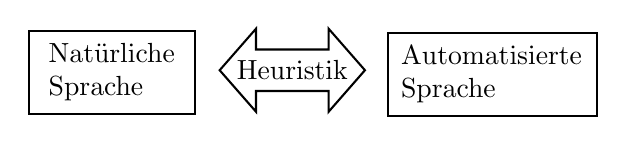
\begin{tikzpicture}[x=0.75pt,y=0.75pt,yscale=-1,xscale=1]
%uncomment if require: \path (0,300); %set diagram left start at 0, and has height of 300

%Shape: Rectangle [id:dp02241090211127661] 
\draw   (81,126) -- (161,126) -- (161,166) -- (81,166) -- cycle ;
%Shape: Rectangle [id:dp20165869726734287] 
\draw   (254,127) -- (355,127) -- (355,167) -- (254,167) -- cycle ;
%Left Right Arrow [id:dp33351638469477385] 
\draw   (173,145) -- (190.5,125) -- (190.5,135) -- (225.5,135) -- (225.5,125) -- (243,145) -- (225.5,165) -- (225.5,155) -- (190.5,155) -- (190.5,165) -- cycle ;

% Text Node
\draw (121,146) node  [align=left] {Natürliche\\Sprache};
% Text Node
\draw (304,147) node  [align=left] {Automatisierte\\Sprache};
% Text Node
\draw (208,145) node  [align=left] {Heuristik};


\end{tikzpicture}
		%\caption{Modellierung}
		%\label{Abb:natSpracheModellierung}
	\end{center}
\end{figure}

\betone{Problem:} Fehlkommunikation\\
Das fehlende Glied ist die Formale Sprache:

\begin{figure}[H] % oder ht!
	\begin{center}
		% This work is licensed under the Creative Commons
% Attribution-NonCommercial-ShareAlike 4.0 International License. To view a copy
% of this license, visit http://creativecommons.org/licenses/by-nc-sa/4.0/ or
% send a letter to Creative Commons, PO Box 1866, Mountain View, CA 94042, USA.

\tikzset{every picture/.style={line width=0.75pt}} %set default line width to 0.75pt        

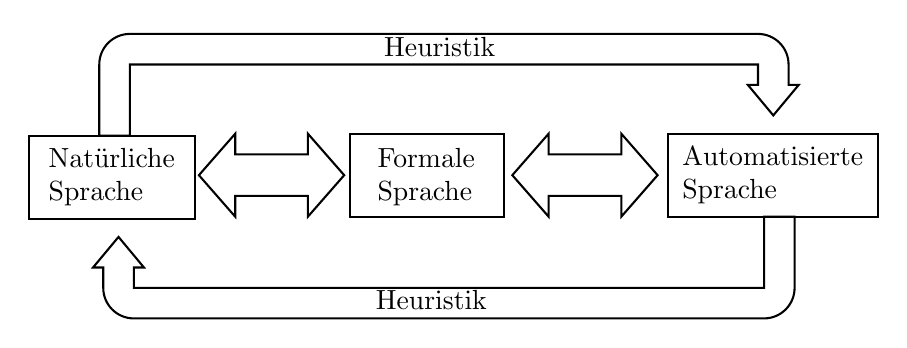
\begin{tikzpicture}[x=0.75pt,y=0.75pt,yscale=-1,xscale=1]
%uncomment if require: \path (0,300); %set diagram left start at 0, and has height of 300

%Shape: Rectangle [id:dp02241090211127661] 
\draw   (81,126) -- (161,126) -- (161,166) -- (81,166) -- cycle ;
%Shape: Rectangle [id:dp20165869726734287] 
\draw   (236,125) -- (310,125) -- (310,165) -- (236,165) -- cycle ;
%Left Right Arrow [id:dp33351638469477385] 
\draw   (163,145) -- (180.5,125) -- (180.5,135) -- (215.5,135) -- (215.5,125) -- (233,145) -- (215.5,165) -- (215.5,155) -- (180.5,155) -- (180.5,165) -- cycle ;
%Shape: Rectangle [id:dp2972974344682269] 
\draw   (389,125) -- (490,125) -- (490,165) -- (389,165) -- cycle ;
%Left Right Arrow [id:dp8197742277124606] 
\draw   (314,145) -- (331.5,125) -- (331.5,135) -- (366.5,135) -- (366.5,125) -- (384,145) -- (366.5,165) -- (366.5,155) -- (331.5,155) -- (331.5,165) -- cycle ;
%U Turn Arrow [id:dp49299810652548426] 
\draw   (115,126) -- (115,91.65) .. controls (115,83.52) and (121.59,76.93) .. (129.72,76.93) -- (432.37,76.93) .. controls (440.5,76.93) and (447.09,83.52) .. (447.09,91.65) -- (447.09,101.47) -- (452,101.47) -- (439.73,116.19) -- (427.47,101.47) -- (432.37,101.47) -- (432.37,91.65) .. controls (432.37,91.65) and (432.37,91.65) .. (432.37,91.65) -- (129.72,91.65) .. controls (129.72,91.65) and (129.72,91.65) .. (129.72,91.65) -- (129.72,126) -- cycle ;
%U Turn Arrow [id:dp46223682559547996] 
\draw   (450,164.93) -- (450,199.28) .. controls (450,207.41) and (443.41,214) .. (435.28,214) -- (131.63,214) .. controls (123.5,214) and (116.91,207.41) .. (116.91,199.28) -- (116.91,189.47) -- (112,189.47) -- (124.27,174.75) -- (136.53,189.47) -- (131.63,189.47) -- (131.63,199.28) .. controls (131.63,199.28) and (131.63,199.28) .. (131.63,199.28) -- (435.28,199.28) .. controls (435.28,199.28) and (435.28,199.28) .. (435.28,199.28) -- (435.28,164.93) -- cycle ;

% Text Node
\draw (121,146) node  [align=left] {Natürliche\\Sprache};
% Text Node
\draw (439.5,145) node  [align=left] {Automatisierte\\Sprache};
% Text Node
\draw (272.5,146) node  [align=left] {Formale\\Sprache};
% Text Node
\draw (279,83) node  [align=left] {Heuristik};
% Text Node
\draw (275,205) node  [align=left] {Heuristik};


\end{tikzpicture}

		%\caption{Modellierung}
		%\label{Abb:natSpracheModellierung}
	\end{center}
\end{figure}

Die Formale Sprache erlaubt Absraktion und Vergleich.
Die automatisierte Sprache ist algorithmisch reichhaltig, aber strukturell arm.
Im Sinne der mathematischen Beschreibung / Modellierung ist ein Modell-Vergleich oft nicht möglich, wenn ich kein abstraktes Modell habe!\nl
Es gibt zwei Wege, Wissen zu erlangen:
\begin{enumerate}
	\item \define{Top Down:} deduktive Methode
	\item \define{Bottom Up:} induktive Methode
\end{enumerate}

Technisches Makro sind symbolische Abkürzungen, z.B. "$\R$".
Im Gegensatz dazu gibt es auch verbale Makros, z.B. "reelle Zahlen".

\subsection{Mengenbasierte Modellierung / strukturelle Modellierung}
\begin{definition}
	Eine \define{Inzidenzstruktur} ist ein Tripel $J=(P,B,I)$ wobei $P,B,I$ Mengen sind mit $I\subseteq P\times B$. 
	Interpretation:
	\begin{itemize}
		\item $P$ ist Menge von Punkten / Points
		\item $B$ ist Menge von Blöcken / Blocks
		\item $I$ Inzidenzrelation (z.B. Lines)
	\end{itemize}
	Für $(p,b)\in I$ schreiben wir auch $pIb$ (incidence) und sagen:\\
	"Der Punkt $p$ inzidiert mit dem Block $b$ in $J$."\\
	Für $p\in P$ sei
	\begin{align*}
		pI:=\set{b\in B\mid pIb}
	\end{align*}
	d.h. die Menge aller mit dem Punkt $p$ inzidierenden Blöcke.\\
	Analog sei für $b\in B$ stets
	\begin{align*}
		Ib:=\set{p\in P\mid pIb}
	\end{align*}
	die Menge aller mit dem Block $b$ inzidierenden Punkte.
\end{definition}

Strukturelle Modellierung ist eine mengenbasierte Modellierung.
Dies ist ein Gegensatz z.B. zur \textbf{Prozedurale Modellierung}.

\begin{beispiel}\
	\begin{itemize}
		\item $P:=$ Eckenmenge eines Würfels
		\item $B:=$ Flächenmenge des Würfels
		\item Inzidenz: Punkt ist Eckpunkt von Würfelfläche
	\end{itemize}
\end{beispiel}

\begin{satz}[Prinzip des doppelten Abzählens]\enter
	Ist $J=(P,B,I)$ endliche Inzidenzstruktur (d.h. $P$ und $B$ endlich), so gilt
	\begin{align*}
		\sum\limits_{p\in P}\# pI=\#I=\sum\limits_{b\in B}\# Ib
	\end{align*}
	Hierbei ist $\#M$ die Anzahl der Elemente von $M$.
\end{satz}

\begin{definition}
	$y$ heißt \define{taktische Konfiguration} der Inzidenzstruktur $J=(P,B,I)$
	\begin{align*}
		:\iff\exists r_y,k_y\in\N:\forall p\in P,\forall b\in B:\# pI=r_y\und\#Ib=k_y
	\end{align*}
\end{definition}

\begin{lemma}
	Sei $y$ taktische Konfiguration von $J=(P,B,I)$. Dann gilt:
	\begin{align*}
		v_y\mal r_y=b_y\mal k_y
		\qquad\mit\qquad
		v_y:=\# P\und b_y:=\#B
	\end{align*}
\end{lemma}

\begin{proof}
	Doppelte Abzählung: 
	\begin{align*}
		v_y\mal r_y=\sum\limits_{p\in P}\underbrace{\# pI}_{=r_y}=\sum\limits_{b\in B}\underbrace{\#Ib}_{=k_y}=b_y\mal r_y
	\end{align*}
\end{proof}


\begin{definition}
	$\big(v_y,r_y;b_y,k_y)$ ist das \define{Parametertupel} von $y$.
	\index{Parametertupel}.
	Das dazu \define{duale Parametertupel} ist $\big(b_y,k_y;v_y,r_y\big)$.
\end{definition}

\begin{beispiel}
	Für unsere Würfelinzidenzstruktur ist das Parametertupel:\\
	(Anzahl der Punkte, Anzahl der Geraden pro Punkt, Anzahl der Geraden, Anzahl der Punkte pro Gerade).
	\begin{enumerate}
		\item Tetraeder (dual Tetraeder): $(4,3;4,3)$ 
		\item Hexader (dual: Oktaeder): $(8,3;6,4)$
		\item Dodekaeder (dual: Ikosaeder): $(20,3;12,5)$
		\item Dreieck: $(3,2;3,2)$ ist auch selbstdual: Dreieck $\leftrightarrow$ Dreiseit
	\end{enumerate}
\end{beispiel}

\begin{beispiel}[Veblen-Young-Configuration]
	\begin{figure}[H] % oder ht!
		\begin{center}
			% This work is licensed under the Creative Commons
% Attribution-NonCommercial-ShareAlike 4.0 International License. To view a copy
% of this license, visit http://creativecommons.org/licenses/by-nc-sa/4.0/ or
% send a letter to Creative Commons, PO Box 1866, Mountain View, CA 94042, USA.



\tikzset{every picture/.style={line width=0.75pt}} %set default line width to 0.75pt        

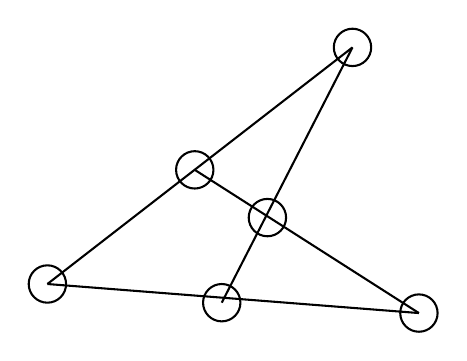
\begin{tikzpicture}[x=0.75pt,y=0.75pt,yscale=-1,xscale=1]
%uncomment if require: \path (0,300); %set diagram left start at 0, and has height of 300

%Shape: Circle [id:dp8256548323361356] 
\draw   (15,144) .. controls (15,139.03) and (19.03,135) .. (24,135) .. controls (28.97,135) and (33,139.03) .. (33,144) .. controls (33,148.97) and (28.97,153) .. (24,153) .. controls (19.03,153) and (15,148.97) .. (15,144) -- cycle ;
%Shape: Circle [id:dp9999136902725693] 
\draw   (162,30) .. controls (162,25.03) and (166.03,21) .. (171,21) .. controls (175.97,21) and (180,25.03) .. (180,30) .. controls (180,34.97) and (175.97,39) .. (171,39) .. controls (166.03,39) and (162,34.97) .. (162,30) -- cycle ;
%Shape: Circle [id:dp7722874472312242] 
\draw   (86,89) .. controls (86,84.03) and (90.03,80) .. (95,80) .. controls (99.97,80) and (104,84.03) .. (104,89) .. controls (104,93.97) and (99.97,98) .. (95,98) .. controls (90.03,98) and (86,93.97) .. (86,89) -- cycle ;
%Shape: Circle [id:dp1591555646648798] 
\draw   (194,158) .. controls (194,153.03) and (198.03,149) .. (203,149) .. controls (207.97,149) and (212,153.03) .. (212,158) .. controls (212,162.97) and (207.97,167) .. (203,167) .. controls (198.03,167) and (194,162.97) .. (194,158) -- cycle ;
%Shape: Circle [id:dp04988684193722637] 
\draw   (121,112) .. controls (121,107.03) and (125.03,103) .. (130,103) .. controls (134.97,103) and (139,107.03) .. (139,112) .. controls (139,116.97) and (134.97,121) .. (130,121) .. controls (125.03,121) and (121,116.97) .. (121,112) -- cycle ;
%Shape: Circle [id:dp15540025125472967] 
\draw   (99,153) .. controls (99,148.03) and (103.03,144) .. (108,144) .. controls (112.97,144) and (117,148.03) .. (117,153) .. controls (117,157.97) and (112.97,162) .. (108,162) .. controls (103.03,162) and (99,157.97) .. (99,153) -- cycle ;
%Straight Lines [id:da9051529769910057] 
\draw    (24,144) -- (171,30) ;


%Straight Lines [id:da9722531504709364] 
\draw    (24,144) -- (203,158) ;


%Straight Lines [id:da879150422612323] 
\draw    (95,89) -- (203,158) ;


%Straight Lines [id:da809884536800273] 
\draw    (171,30) -- (108,153) ;

\end{tikzpicture}

			\caption{Veblen-Young-Konfiguration: $(6,2;4,3)$}
			%\label{Abb:natSpracheModellierung}
		\end{center}
	\end{figure}
	\begin{figure}[H] % oder ht!
		\begin{center}
			% This work is licensed under the Creative Commons
% Attribution-NonCommercial-ShareAlike 4.0 International License. To view a copy
% of this license, visit http://creativecommons.org/licenses/by-nc-sa/4.0/ or
% send a letter to Creative Commons, PO Box 1866, Mountain View, CA 94042, USA.


\tikzset{every picture/.style={line width=0.75pt}} %set default line width to 0.75pt        

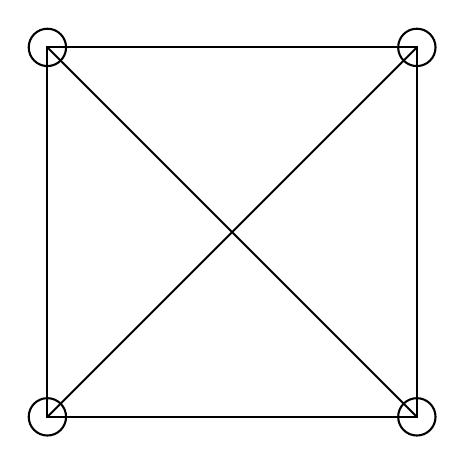
\begin{tikzpicture}[x=0.75pt,y=0.75pt,yscale=-1,xscale=1]
%uncomment if require: \path (0,300); %set diagram left start at 0, and has height of 300

%Shape: Square [id:dp9706132534648327] 
\draw   (201,62) -- (379,62) -- (379,240) -- (201,240) -- cycle ;
%Straight Lines [id:da9618724140233941] 
\draw    (201,62) -- (379,240) ;


%Straight Lines [id:da3907949926394131] 
\draw    (379,62) -- (201,240) ;


%Shape: Circle [id:dp5133007782867983] 
\draw   (192,62) .. controls (192,57.03) and (196.03,53) .. (201,53) .. controls (205.97,53) and (210,57.03) .. (210,62) .. controls (210,66.97) and (205.97,71) .. (201,71) .. controls (196.03,71) and (192,66.97) .. (192,62) -- cycle ;
%Shape: Circle [id:dp3477876429055702] 
\draw   (192,240) .. controls (192,235.03) and (196.03,231) .. (201,231) .. controls (205.97,231) and (210,235.03) .. (210,240) .. controls (210,244.97) and (205.97,249) .. (201,249) .. controls (196.03,249) and (192,244.97) .. (192,240) -- cycle ;
%Shape: Circle [id:dp36747093980837164] 
\draw   (370,240) .. controls (370,235.03) and (374.03,231) .. (379,231) .. controls (383.97,231) and (388,235.03) .. (388,240) .. controls (388,244.97) and (383.97,249) .. (379,249) .. controls (374.03,249) and (370,244.97) .. (370,240) -- cycle ;
%Shape: Circle [id:dp00705377401053342] 
\draw   (370,62) .. controls (370,57.03) and (374.03,53) .. (379,53) .. controls (383.97,53) and (388,57.03) .. (388,62) .. controls (388,66.97) and (383.97,71) .. (379,71) .. controls (374.03,71) and (370,66.97) .. (370,62) -- cycle ;

\end{tikzpicture}

			\caption{duela Veblen-Young-Konfiguration: $(4,3;6,2)$}
			%\label{Abb:natSpracheModellierung}
		\end{center}
	\end{figure}	
\end{beispiel}

\begin{beispiel}
	Berühmte taktische Konfiguation ist $(10,3;10,3)$.\\
	Sei $[n]:=\set{1,\ldots,n}$ für $n\in\N$ und $\ul{n}:=\set{0,\ldots,n-1}$.
	Sei $\begin{pmatrix}
		M\\k
	\end{pmatrix}:=\set{X\subseteq M\mid\#X=k}$ für $M$ Menge.
	Dann gilt $\#\begin{pmatrix}
		M\\k
	\end{pmatrix}=\begin{pmatrix}
		\#M\\k
	\end{pmatrix}$.
	Seien $i,j,n\in\N$ mit $i\leq j\leq n$.
	Setze
	\begin{align*}
		J^n_{(i,j)}&:=\klammern{\begin{pmatrix}
			[n]\\i
		\end{pmatrix},\begin{pmatrix}
			[n]\\ j
		\end{pmatrix},I^n_{(i,j)}}\qquad\mit\\
		I^n_{(i,j)}&:=\set{(p,b)\in\begin{pmatrix}
			[n]\\ i
		\end{pmatrix}\times\begin{pmatrix}
			[n]\\j
		\end{pmatrix}\mid p\subseteq b}
	\end{align*}
	Dann ist $J^n_{(i,j)}$ taktische Konfiguration mit dem Parametertupel
	\begin{align*}
		\klammern{
		\begin{pmatrix}
			n\\i
		\end{pmatrix},
		\begin{pmatrix}
			n-i\\j-i
		\end{pmatrix},
		\begin{pmatrix}
			n\\j
		\end{pmatrix},
		\begin{pmatrix}
			j\\i
		\end{pmatrix}
		}
	\end{align*}
	Wann ist dies gleich $(10,3;10,3)$?
	Oder gleich $(4,3;6,2)$? Antwort:
	\begin{align*}
		(4,3;6,2)=\klammern{\begin{pmatrix}
			4\\1
		\end{pmatrix},\begin{pmatrix}
			4-1\\2-1
		\end{pmatrix},
		\begin{pmatrix}
			4\\2
		\end{pmatrix},
		\begin{pmatrix}
			2\\1
		\end{pmatrix}}
	\end{align*}
	dh. $(i,j,n)=(1,2,4)$.
\end{beispiel}





